\documentclass[11pt,a4paper]{report}
\usepackage[textwidth=37em,vmargin=30mm]{geometry}
\usepackage{calc,xunicode,amsmath,amssymb,paralist,enumitem,tabu,booktabs,datetime2,xeCJK,xeCJKfntef,listings}
\usepackage{tocloft,fancyhdr,tcolorbox,xcolor,graphicx,eso-pic,xltxtra,xelatexemoji}

\newcommand{\envyear}[0]{2025}
\newcommand{\envdatestr}[0]{2025-02-01}
\newcommand{\envfinaldir}[0]{webdb/2025/20250201/final}

\usepackage[hidelinks]{hyperref}
\hypersetup{
    colorlinks=false,
    pdfpagemode=FullScreen,
    pdftitle={Web Digest - \envdatestr}
}

\setlength{\cftbeforechapskip}{10pt}
\renewcommand{\cftchapfont}{\rmfamily\bfseries\large\raggedright}
\setlength{\cftbeforesecskip}{2pt}
\renewcommand{\cftsecfont}{\sffamily\small\raggedright}

\setdefaultleftmargin{2em}{2em}{1em}{1em}{1em}{1em}

\usepackage{xeCJK,xeCJKfntef}
\xeCJKsetup{PunctStyle=plain,RubberPunctSkip=false,CJKglue=\strut\hskip 0pt plus 0.1em minus 0.05em,CJKecglue=\strut\hskip 0.22em plus 0.2em}
\XeTeXlinebreaklocale "zh"
\XeTeXlinebreakskip = 0pt


\setmainfont{Brygada 1918}
\setromanfont{Brygada 1918}
\setsansfont{IBM Plex Sans}
\setmonofont{JetBrains Mono NL}
\setCJKmainfont{Noto Serif CJK SC}
\setCJKromanfont{Noto Serif CJK SC}
\setCJKsansfont{Noto Sans CJK SC}
\setCJKmonofont{Noto Sans CJK SC}

\setlength{\parindent}{0pt}
\setlength{\parskip}{8pt}
\linespread{1.15}

\lstset{
	basicstyle=\ttfamily\footnotesize,
	numbersep=5pt,
	backgroundcolor=\color{black!5},
	showspaces=false,
	showstringspaces=false,
	showtabs=false,
	tabsize=2,
	captionpos=b,
	breaklines=true,
	breakatwhitespace=true,
	breakautoindent=true,
	linewidth=\textwidth
}






\newcommand{\coverpic}[2]{
    % argv: itemurl, authorname
    Cover photo by #2~~(\href{#1}{#1})
}
\newcommand{\makeheader}[0]{
    \begin{titlepage}
        % \newgeometry{hmargin=15mm,tmargin=21mm,bmargin=12mm}
        \begin{center}
            
            \rmfamily\scshape
            \fontspec{BaskervilleF}
            \fontspec{Old Standard}
            \fontsize{59pt}{70pt}\selectfont
            WEB\hfill DIGEST
            
            \vfill
            % \vskip 30pt
            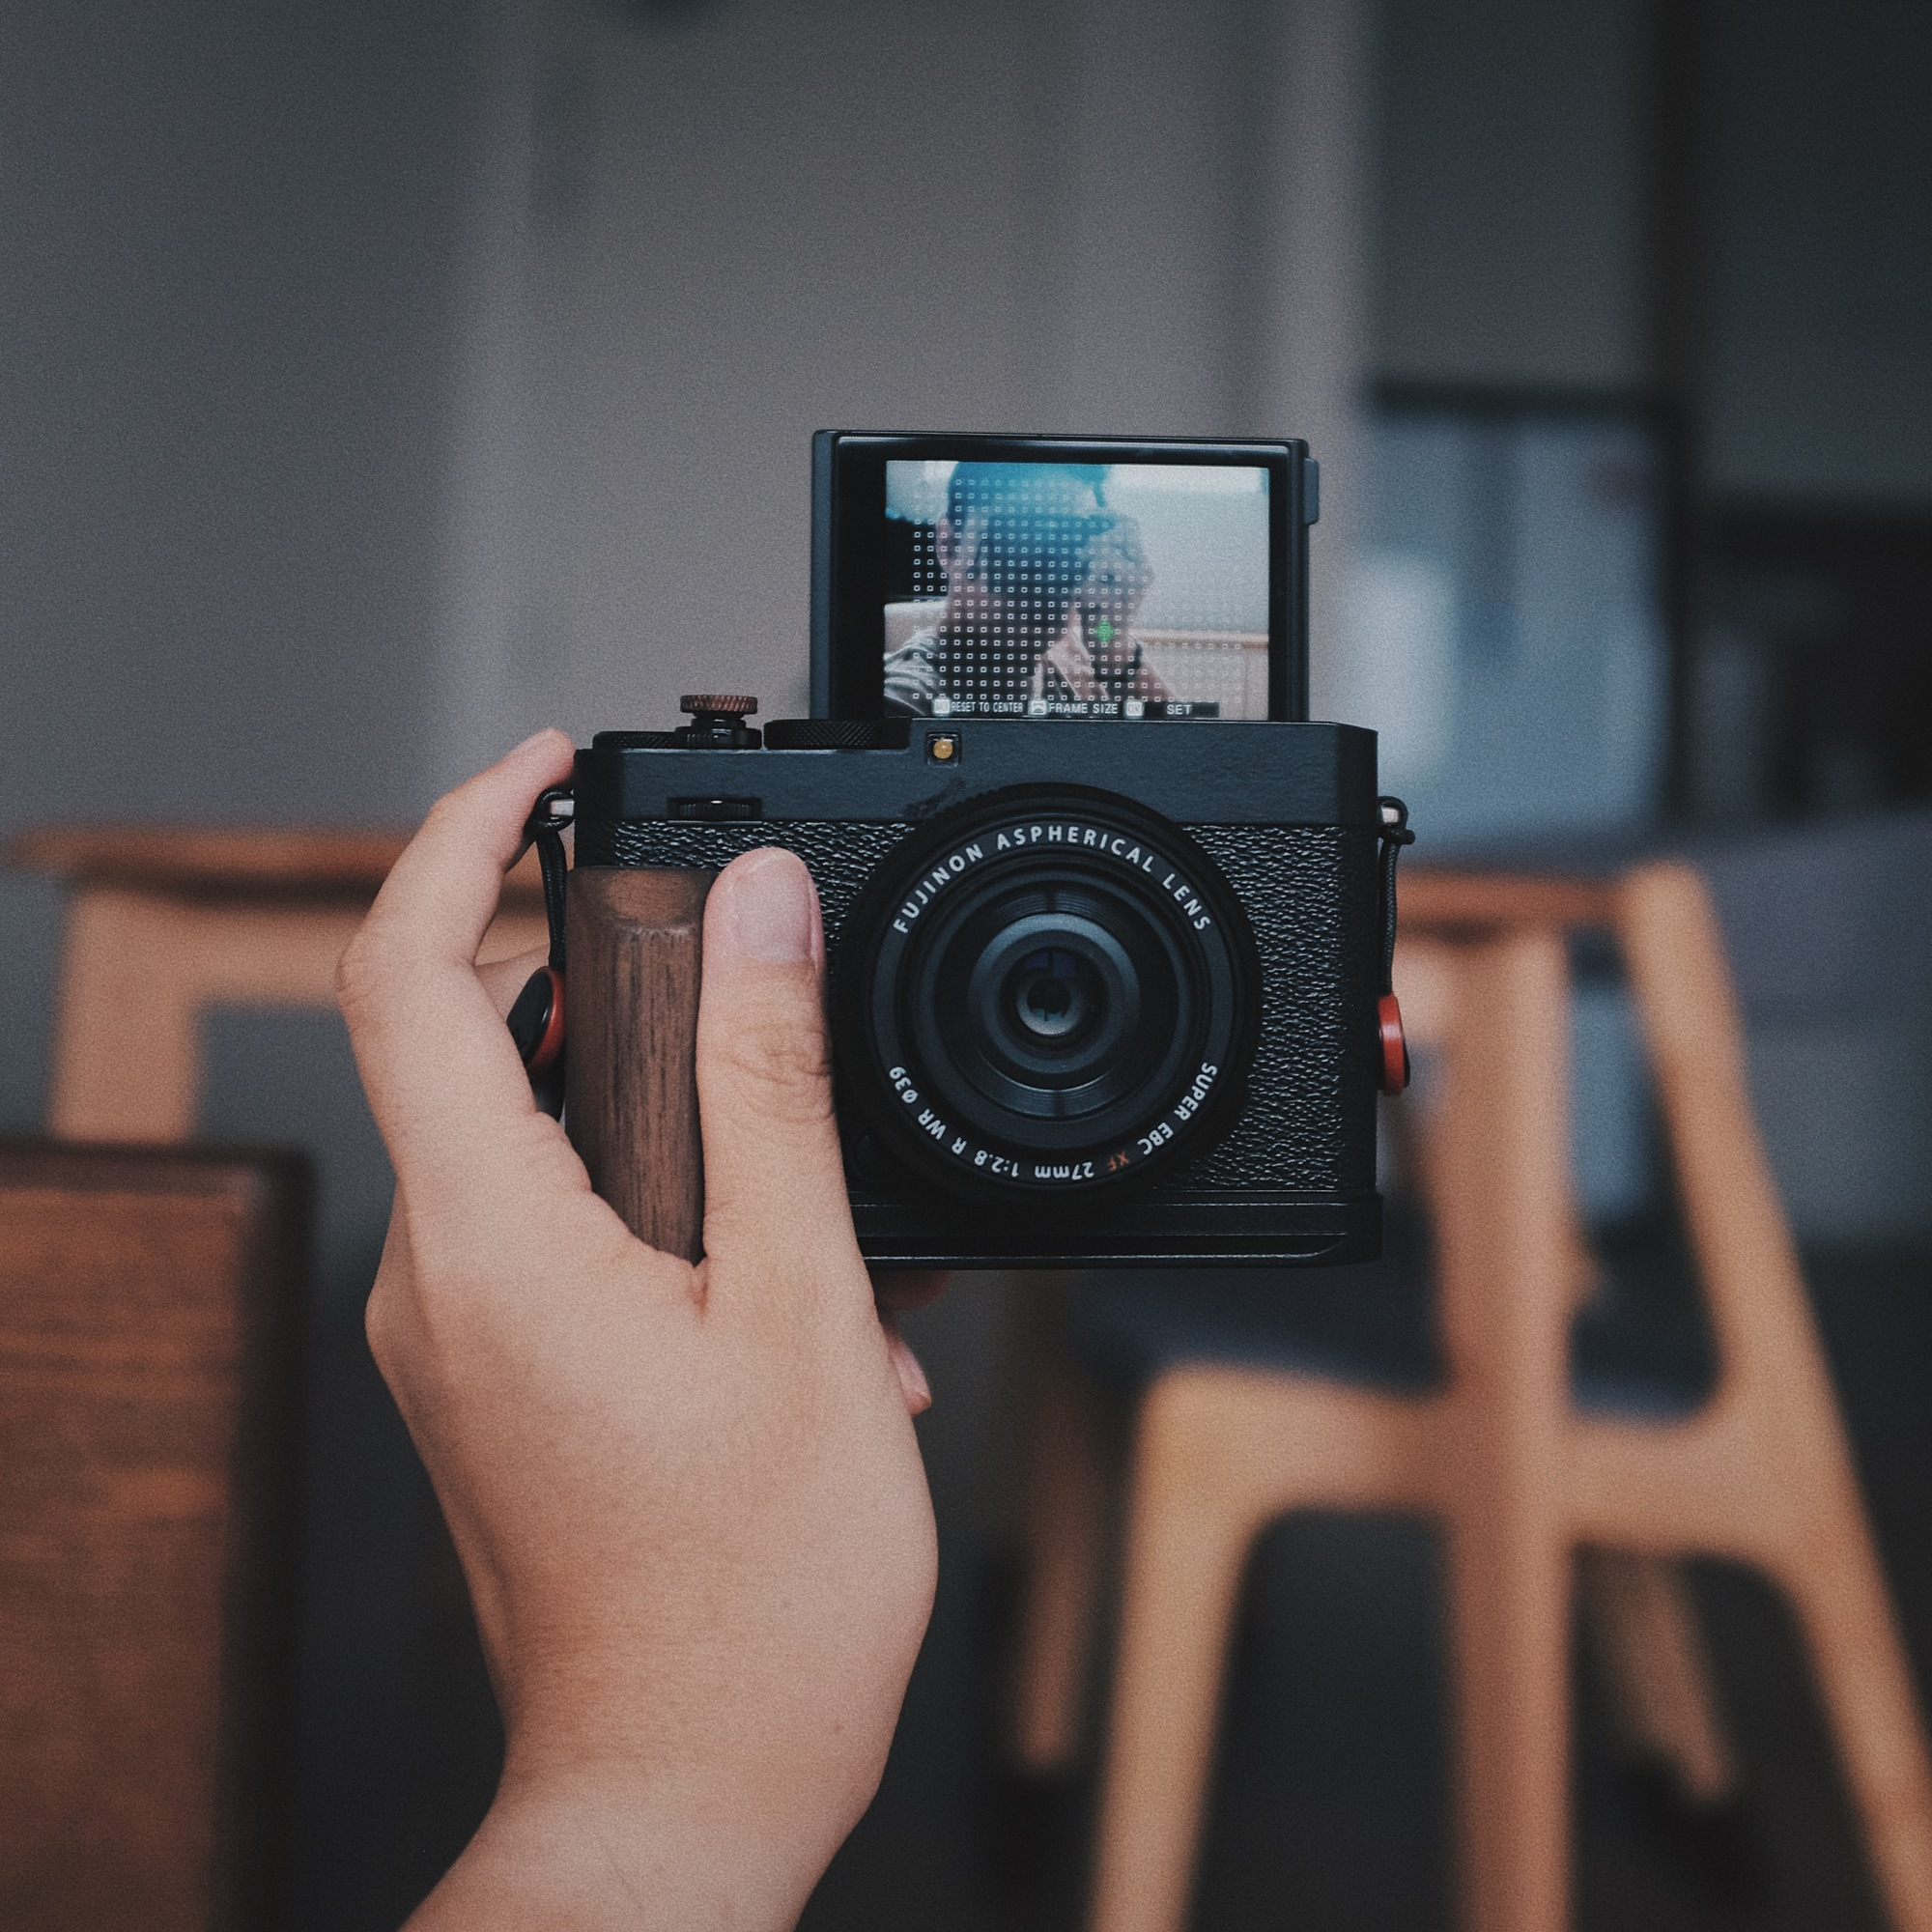
\includegraphics[width=\linewidth]{\envfinaldir/coverpic-prod.jpg}\par
            % \vskip 30pt
            \vfill

            \normalsize\rmfamily\scshape
            \copyright{} The Web Digest Project \hfill\large \envdatestr
        \end{center}
    \end{titlepage}
    % \restoregeometry
}
\newcommand{\simplehref}[1]{%
    \textcolor{blue!80!green}{\href{#1}{#1}}%
}
\renewcommand{\contentsname}{\center\Huge\sffamily\bfseries Contents\par\vskip 20pt}
\newcounter{ipartcounter}
\setcounter{ipartcounter}{0}
\newcommand{\ipart}[1]{
    % \vskip 20pt
    \clearpage
    \stepcounter{ipartcounter}
    \phantomsection
    \addcontentsline{toc}{chapter}{#1}
    % \begin{center}
    %     \Huge
    %     \sffamily\bfseries
    %     #1
    % \end{center}
    % \vskip 20pt plus 7pt
}
\newcounter{ichaptercounter}
\setcounter{ichaptercounter}{0}
\newcommand{\ichapter}[1]{
    % \vskip 20pt
    \clearpage
    \stepcounter{ichaptercounter}
    \phantomsection
    \addcontentsline{toc}{section}{\numberline{\arabic{ichaptercounter}}#1}
    \begin{center}
        \Huge
        \sffamily\bfseries
        #1
    \end{center}
    \vskip 20pt plus 7pt
}
\newcommand{\entrytitlefont}[1]{\subsection*{\raggedright\Large\sffamily\bfseries#1}}
\newcommand{\entryitemGeneric}[2]{
    % argv: title, url
    \parbox{\linewidth}{
        \entrytitlefont{#1}\par\vskip 5pt
        \footnotesize\ttfamily\mdseries
        \simplehref{#2}
    }\vskip 11pt plus 11pt minus 1pt
}
\newcommand{\entryitemGithub}[3]{
    % argv: title, url, desc
    \parbox{\linewidth}{
        \entrytitlefont{#1}\par\vskip 5pt
        \footnotesize\ttfamily\mdseries
        \simplehref{#2}\par\vskip 5pt
        \small\rmfamily\mdseries#3
    }\vskip 11pt plus 11pt minus 1pt
}
\newcommand{\entryitemAp}[3]{
    % argv: title, url, desc
    \parbox{\linewidth}{
        \entrytitlefont{#1}\par\vskip 5pt
        \footnotesize\ttfamily\mdseries
        \simplehref{#2}\par\vskip 5pt
        \small\rmfamily\mdseries#3
    }\vskip 11pt plus 11pt minus 1pt
}
\newcommand{\entryitemHackernews}[3]{
    % argv: title, hnurl, rawurl
    % \parbox{\linewidth}{
    %     \entrytitlefont{#1}\par\vskip 5pt
    %     \footnotesize\ttfamily\mdseries
    %     \simplehref{#3}\par
    %     \textcolor{black!50}{\href{#2}{#2}}
    % }\vskip 11pt plus 11pt minus 1pt
    \begin{minipage}{\linewidth}
            \entrytitlefont{#1}\par\vskip 5pt
            \footnotesize\ttfamily\mdseries
            \simplehref{#3}\par
            \textcolor{black!50}{\href{#2}{#2}}
    \end{minipage}\par\vskip 11pt plus 11pt minus 1pt
}







\begin{document}

\makeheader

\tableofcontents\clearpage




\ipart{Developers}
\ichapter{Hacker News}
\entryitemTwoLinks{Tesla Paid Zero Federal Income Tax in 2024, Despite \$2.3B in Income}{https://news.ycombinator.com/item?id=42893365}{https://truthout.org/articles/tesla-paid-zero-federal-income-tax-in-2024-despite-2-3-billion-in-income/}

\entryitemTwoLinks{Musk aides lock government workers out of computer systems at US agency}{https://news.ycombinator.com/item?id=42892278}{https://www.reuters.com/world/us/musk-aides-lock-government-workers-out-computer-systems-us-agency-sources-say-2025-01-31/}

\entryitemTwoLinks{Add "fucking" to your Google searches to neutralize AI summaries}{https://news.ycombinator.com/item?id=42892191}{https://gizmodo.com/add-fcking-to-your-google-searches-to-neutralize-ai-summaries-2000557710}

\entryitemTwoLinks{GenAI Art Is the Least Imaginative Use of AI Imaginable}{https://news.ycombinator.com/item?id=42891821}{https://hai.stanford.edu/news/ge-wang-genai-art-least-imaginative-use-ai-imaginable}

\entryitemTwoLinks{US government agency argues that money isn't property–so it can take yours}{https://news.ycombinator.com/item?id=42891724}{https://reason.com/2025/01/31/the-government-says-money-isnt-property-so-it-can-take-yours/}

\entryitemTwoLinks{Elite on the 6502: The original 6502 assembly source, heavily commented}{https://news.ycombinator.com/item?id=42891200}{https://elite.bbcelite.com/}

\entryitemTwoLinks{Instagram and Facebook Blocked and Hid Abortion Pill Providers' Posts}{https://news.ycombinator.com/item?id=42891148}{https://www.nytimes.com/2025/01/23/technology/instagram-facebook-abortion-pill-providers.html}

\entryitemTwoLinks{Bypass DeepSeek censorship by speaking in hex}{https://news.ycombinator.com/item?id=42891042}{https://substack.com/home/post/p-156004330}

\entryitemTwoLinks{Meta in talks to reincorporate in Texas or another state, WSJ reports}{https://news.ycombinator.com/item?id=42890960}{https://www.reuters.com/technology/meta-talks-reincorporate-texas-or-another-state-exit-delaware-wsj-reports-2025-01-31/}

\entryitemTwoLinks{OpenAI O3-Mini}{https://news.ycombinator.com/item?id=42890627}{https://openai.com/index/openai-o3-mini/}

\entryitemTwoLinks{Three AM 911 call, 9 AM salesman}{https://news.ycombinator.com/item?id=42889777}{https://a.wholelottanothing.org/when-everything-becomes-a-profit-center/}

\entryitemTwoLinks{Living with Nausea: My Story in Six Charts}{https://news.ycombinator.com/item?id=42889700}{https://www.c82.net/blog/?id=96}

\entryitemTwoLinks{Show HN: Uscope, a new Linux debugger written from scratch}{https://news.ycombinator.com/item?id=42889407}{https://github.com/jcalabro/uscope}

\entryitemTwoLinks{Apple files emergency motion to become defendant in US vs. Google [pdf]}{https://news.ycombinator.com/item?id=42889297}{https://storage.courtlistener.com/recap/gov.uscourts.dcd.223205/gov.uscourts.dcd.223205.1158.0\_1.pdf}

\entryitemTwoLinks{How to Train an AI Image Model on Yourself}{https://news.ycombinator.com/item?id=42889236}{https://www.coryzue.com/writing/make-ai-pictures-of-yourself/}

\entryitemTwoLinks{RamaLama}{https://news.ycombinator.com/item?id=42887939}{https://github.com/containers/ramalama}

\entryitemTwoLinks{Ear muscle we thought humans didn't use activates when people listen hard}{https://news.ycombinator.com/item?id=42886867}{https://www.frontiersin.org/news/2025/01/31/ear-muscle-wiggling-ears-activates-listening-frontiers-neuroscience}

\entryitemTwoLinks{Taking a \$15 Casio F91W 5km underwater}{https://news.ycombinator.com/item?id=42886718}{https://www.watchesofespionage.com/blogs/woe-dispatch/casio-f91w-diving-underwater-pressure-test}

\entryitemTwoLinks{Llama.cpp supports Vulkan. why doesn't Ollama?}{https://news.ycombinator.com/item?id=42886680}{https://github.com/ollama/ollama/pull/5059}

\entryitemTwoLinks{NSF starts vetting all grants to comply with executive orders}{https://news.ycombinator.com/item?id=42886661}{https://www.science.org/content/article/exclusive-nsf-starts-vetting-all-grants-comply-trump-s-orders}\ichapter{Phoronix}
\entryitemGeneric{\hskip 0pt{}TLB Flushing Scalability Optimizations Merged For Linux 6.14 To Benefit AMD / Intel CPUs}{https://www.phoronix.com/news/Linux-6.14-TLB-Flush-Scalable}

\entryitemGeneric{\hskip 0pt{}GNOME 48 Switches Over To "Adwaita Sans" As Default Font}{https://www.phoronix.com/news/GNOME-48-Adwaita-Sans}

\entryitemGeneric{\hskip 0pt{}The Compelling AVX-512 Performance Advantage On AMD EPYC 9005 "Turin"}{https://www.phoronix.com/review/amd-epyc-turin-avx512}

\entryitemGeneric{\hskip 0pt{}Servo Aims For Shadow DOM \& Improved Embedding API In 2025}{https://www.phoronix.com/news/Servo-Roadmap-2025}

\entryitemGeneric{\hskip 0pt{}KVM Enhancements Within The Linux 6.14 Kernel}{https://www.phoronix.com/news/Linux-6.14-KVM}

\entryitemGeneric{\hskip 0pt{}Chromium Embedded Framework "CEF" Seeing Progress On Wayland Support}{https://www.phoronix.com/news/Chromium-CEF-Wayland-Progress}

\entryitemGeneric{\hskip 0pt{}FUSE Hooks Up With IO\_uring For Greater Performance Potential In Linux 6.14}{https://www.phoronix.com/news/Linux-6.14-FUSE}

\entryitemGeneric{\hskip 0pt{}NVIDIA VFIO Driver Prepares For Blackwell With Linux 6.14}{https://www.phoronix.com/news/Linux-6.14-VFIO}

\entryitemGeneric{\hskip 0pt{}Mesa 25.0-rc1 Released With Initial AMD RDNA4 Support, Vulkan 1.4 \& Other New Extensions}{https://www.phoronix.com/news/Mesa-25.0-rc1}\ichapter{Dribbble}
\entryitemGeneric{\hskip 0pt{}Atlantic Pickleball Club}{https://dribbble.com/shots/25558009-Atlantic-Pickleball-Club}

\entryitemGeneric{\hskip 0pt{}Stellar}{https://dribbble.com/shots/25559656-Stellar}

\entryitemGeneric{\hskip 0pt{}Wizard Logo}{https://dribbble.com/shots/25559490-Wizard-Logo}

\entryitemGeneric{\hskip 0pt{}Shuttle Robotics}{https://dribbble.com/shots/25557675-Shuttle-Robotics}

\entryitemGeneric{\hskip 0pt{}Real Estate Web Design}{https://dribbble.com/shots/25551949-Real-Estate-Web-Design}

\entryitemGeneric{\hskip 0pt{}Puzzle Fintech Website Design}{https://dribbble.com/shots/25501121-Puzzle-Fintech-Website-Design}

\entryitemGeneric{\hskip 0pt{}Columbus Bound®}{https://dribbble.com/shots/25550878-Columbus-Bound}

\entryitemGeneric{\hskip 0pt{}Vista Brand Identity}{https://dribbble.com/shots/25402719-Vista-Brand-Identity}

\entryitemGeneric{\hskip 0pt{}Team Heyo}{https://dribbble.com/shots/25539716-Team-Heyo}

\entryitemGeneric{\hskip 0pt{}Top of the World™ Hunt Club}{https://dribbble.com/shots/25545423-Top-of-the-World-Hunt-Club}

\entryitemGeneric{\hskip 0pt{}DeepSeek logo redesign}{https://dribbble.com/shots/25543483-DeepSeek-logo-redesign}

\entryitemGeneric{\hskip 0pt{}Abstro 8}{https://dribbble.com/shots/25546566-Abstro-8}

\entryitemGeneric{\hskip 0pt{}HappyDev - Logo Design (sold)}{https://dribbble.com/shots/25544140-HappyDev-Logo-Design-sold}

\entryitemGeneric{\hskip 0pt{}Illustration set}{https://dribbble.com/shots/25540370-Illustration-set}

\entryitemGeneric{\hskip 0pt{}VCC Unused Logo Concept - V6}{https://dribbble.com/shots/25543565-VCC-Unused-Logo-Concept-V6}

\entryitemGeneric{\hskip 0pt{}Year of the Snake}{https://dribbble.com/shots/25527312-Year-of-the-Snake}

\entryitemGeneric{\hskip 0pt{}Apparel}{https://dribbble.com/shots/25538973-Apparel}

\entryitemGeneric{\hskip 0pt{}2024 Logo Design Recap Pt.1}{https://dribbble.com/shots/25534698-2024-Logo-Design-Recap-Pt-1}

\entryitemGeneric{\hskip 0pt{}B}{https://dribbble.com/shots/25536900-B}

\entryitemGeneric{\hskip 0pt{}De Nieuwe Gemeente - Church Brand}{https://dribbble.com/shots/25537128-De-Nieuwe-Gemeente-Church-Brand}

\entryitemGeneric{\hskip 0pt{}Speed Test App Ui Design}{https://dribbble.com/shots/25535763-Speed-Test-App-Ui-Design}

\entryitemGeneric{\hskip 0pt{}Plexo mobile app}{https://dribbble.com/shots/25534405-Plexo-mobile-app}

\entryitemGeneric{\hskip 0pt{}VCC Unused Logo Concept V5}{https://dribbble.com/shots/25534846-VCC-Unused-Logo-Concept-V5}

\entryitemGeneric{\hskip 0pt{}Illustration set}{https://dribbble.com/shots/25522996-Illustration-set}


\ipart{Developers~~~~(zh-Hans)}
\ichapter{Solidot}
\entryitemGeneric{\hskip 0pt{}朱诺号在木卫一上记录到至今最强的火山活动}{https://www.solidot.org/story?sid=80455}

\entryitemGeneric{\hskip 0pt{}新发现小行星有 1/83 的概率在 2032 年撞击地球}{https://www.solidot.org/story?sid=80454}

\entryitemGeneric{\hskip 0pt{}库克告诉张忠谋英特尔不知道如何代工芯片}{https://www.solidot.org/story?sid=80453}

\entryitemGeneric{\hskip 0pt{}巴塞尔税务机关因域名错误不得不购买巴哈马域名}{https://www.solidot.org/story?sid=80452}

\entryitemGeneric{\hskip 0pt{}美国版权局称 AI 辅助作品如果包含足够的人类创意可获得版权保护}{https://www.solidot.org/story?sid=80451}

\entryitemGeneric{\hskip 0pt{}LibreOffice 下载量突破 4 亿}{https://www.solidot.org/story?sid=80450}

\entryitemGeneric{\hskip 0pt{}Debian 项目停止在 X 上发推}{https://www.solidot.org/story?sid=80449}

\entryitemGeneric{\hskip 0pt{}Douglas Engelbart 诞辰 100 周年}{https://www.solidot.org/story?sid=80448}

\entryitemGeneric{\hskip 0pt{}Meta 短暂禁止用户发表任何涉及 Linux 的帖子}{https://www.solidot.org/story?sid=80447}

\entryitemGeneric{\hskip 0pt{}腾讯游戏《三角洲行动》被发现会修改用户 CPU 调度和性能释放策略}{https://www.solidot.org/story?sid=80446}

\entryitemGeneric{\hskip 0pt{}心脏病是美国的第一死因}{https://www.solidot.org/story?sid=80445}

\entryitemGeneric{\hskip 0pt{}公共图书馆能给人们的生活带来积极影响}{https://www.solidot.org/story?sid=80444}\ichapter{V2EX}
\entryitemGeneric{\hskip 0pt{}[OpenAI] openai 上线了 o3-mini}{https://www.v2ex.com/t/1108468}

\entryitemGeneric{\hskip 0pt{}[问与答] 2025 年 Windows 和 iPhone 互联性怎么样?}{https://www.v2ex.com/t/1108466}

\entryitemGeneric{\hskip 0pt{}[OpenAI] 有没有大佬告诉我 deepseek 的图片到底是如何识别的}{https://www.v2ex.com/t/1108465}

\entryitemGeneric{\hskip 0pt{}[程序员] 不知道为什么,我很厌恶 map()}{https://www.v2ex.com/t/1108464}

\entryitemGeneric{\hskip 0pt{}[问与答] 现在安卓模拟器里脚本用啥写好呢?}{https://www.v2ex.com/t/1108463}

\entryitemGeneric{\hskip 0pt{}[Telegram] tg 号突然没了, 有类似的软件推荐吗}{https://www.v2ex.com/t/1108461}

\entryitemGeneric{\hskip 0pt{}[分享创造] cursor 哥一小时速成的网站}{https://www.v2ex.com/t/1108460}

\entryitemGeneric{\hskip 0pt{}[微软] outlook 就很神奇,会收到收件人不是我的邮件和发件人是我的邮件}{https://www.v2ex.com/t/1108459}

\entryitemGeneric{\hskip 0pt{}[酷工作] 招聘| 3-5 年前端开发,远程兼职,后期可全职 15-25K}{https://www.v2ex.com/t/1108458}

\entryitemGeneric{\hskip 0pt{}[程序员] 用 C\# 类型系统做了个 Brainfuck 编译器}{https://www.v2ex.com/t/1108457}

\entryitemGeneric{\hskip 0pt{}[宽带症候群] 过户一个 上海联通 1000/200 月租 49 的宽带}{https://www.v2ex.com/t/1108456}

\entryitemGeneric{\hskip 0pt{}[生活] 从童年保留至今的阴影:``去敬一圈酒''}{https://www.v2ex.com/t/1108454}

\entryitemGeneric{\hskip 0pt{}[随想] 刚到公司准备上班,怎么更有意义的过好这一天呢?}{https://www.v2ex.com/t/1108452}

\entryitemGeneric{\hskip 0pt{}[问与答] 小主机/小型服务器推荐}{https://www.v2ex.com/t/1108451}

\entryitemGeneric{\hskip 0pt{}[Visual Studio Code] 2025 年了,有哪些 vscode 插件是你觉得应该卸载的?}{https://www.v2ex.com/t/1108450}

\entryitemGeneric{\hskip 0pt{}[问与答] 有优雅的俩人, mac 和 win 的共用使用方案吗?}{https://www.v2ex.com/t/1108449}

\entryitemGeneric{\hskip 0pt{}[随想] 越大越觉得孤单}{https://www.v2ex.com/t/1108448}

\entryitemGeneric{\hskip 0pt{}[问与答] 找到系统变卡的原因了}{https://www.v2ex.com/t/1108447}

\entryitemGeneric{\hskip 0pt{}[问与答] 刚进入职场的程序员应该在哪些方面提升自己,如何看好未来的路}{https://www.v2ex.com/t/1108446}

\entryitemGeneric{\hskip 0pt{}[YouTube] 有哪些 Youtube 下载工具(带 WebUI 的容器)还可用?}{https://www.v2ex.com/t/1108445}

\entryitemGeneric{\hskip 0pt{}[分享创造] 一场独立开发的刻意练习之旅 - \#1 密码学可视化工具 cipher4.fun}{https://www.v2ex.com/t/1108444}

\entryitemGeneric{\hskip 0pt{}[宽带症候群] 大过节的,跨网 QOS 疑似取消}{https://www.v2ex.com/t/1108443}

\entryitemGeneric{\hskip 0pt{}[问与答] 过年,亲戚待在一起,是如何打发时间的?}{https://www.v2ex.com/t/1108442}

\entryitemGeneric{\hskip 0pt{}[问与答] 求推荐千元以下的蓝牙耳机}{https://www.v2ex.com/t/1108441}

\entryitemGeneric{\hskip 0pt{}[Apple] 求助 请问收到 苹果的 Billing Problem 之前订阅了 2 个月的油管}{https://www.v2ex.com/t/1108440}

\entryitemGeneric{\hskip 0pt{}[分享发现] 一个冷知识:知乎首页第 2 个问答,必然含有广告}{https://www.v2ex.com/t/1108439}

\entryitemGeneric{\hskip 0pt{}[macOS] macos 能否针对某些 App 指定另一个 HOME 目录?}{https://www.v2ex.com/t/1108437}

\entryitemGeneric{\hskip 0pt{}[分享发现] deepseek 交流群}{https://www.v2ex.com/t/1108435}

\entryitemGeneric{\hskip 0pt{}[分享发现] 都在加入 ai 功能,地图软件为什么不加入大模型功能呢?}{https://www.v2ex.com/t/1108431}

\entryitemGeneric{\hskip 0pt{}[问与答] 2025 年,有什么可参考的和 AI 交互的组件库或者规范手册来指导怎么构建 AI 应用吗?}{https://www.v2ex.com/t/1108430}

\entryitemGeneric{\hskip 0pt{}[VPS] 小众 vps 求推荐}{https://www.v2ex.com/t/1108429}

\entryitemGeneric{\hskip 0pt{}[Chrome] 求推荐 chrome 插件-支持自动页面跳转}{https://www.v2ex.com/t/1108428}

\entryitemGeneric{\hskip 0pt{}[分享创造] 开发了一个 ai 生成动漫图片的网站}{https://www.v2ex.com/t/1108427}

\entryitemGeneric{\hskip 0pt{}[问与答] 不论国内国外,你们的 50 系显卡买到了吗}{https://www.v2ex.com/t/1108425}

\entryitemGeneric{\hskip 0pt{}[随想] 发现错了马上改,是最重要的人生法则。}{https://www.v2ex.com/t/1108424}

\entryitemGeneric{\hskip 0pt{}[远程工作] \# 算法工程师 | 远程兼职}{https://www.v2ex.com/t/1108423}

\entryitemGeneric{\hskip 0pt{}[问与答] 如何禁止 Windows 10 精简的组件,在 Windows Update 更新后再次安装?}{https://www.v2ex.com/t/1108422}

\entryitemGeneric{\hskip 0pt{}[前端开发] webstorm 和 vscode,你选哪个:}{https://www.v2ex.com/t/1108420}

\entryitemGeneric{\hskip 0pt{}[问与答] 回娘家真没意思}{https://www.v2ex.com/t/1108419}

\entryitemGeneric{\hskip 0pt{}[问与答] 如何 RSS 推特和贴吧}{https://www.v2ex.com/t/1108418}

\entryitemGeneric{\hskip 0pt{}[NVIDIA] 以前 NVIDIA 两代间的显卡有像 4080->5080 提升幅度这么小(综合看只有 10\%)的吗? 5080 性价比真的非常低吗?最近制作游戏想升级下显卡, 4080 还是 5080 更值}{https://www.v2ex.com/t/1108417}

\entryitemGeneric{\hskip 0pt{}[VPS] 腾讯云 VPS 到期了,资源也释放了,请问还有什么办法恢复吗?}{https://www.v2ex.com/t/1108416}

\entryitemGeneric{\hskip 0pt{}[Android] 大家新年好!请问是否存在一款格式化指定数字的 Android APP 呢?输出效果类似于 printf 那种?}{https://www.v2ex.com/t/1108415}

\entryitemGeneric{\hskip 0pt{}[问与答] 自建私用 DNS 递归服务器无法解决的问题}{https://www.v2ex.com/t/1108414}

\entryitemGeneric{\hskip 0pt{}[硬件] 去日本旅游带块 5090 回来能回多少?}{https://www.v2ex.com/t/1108412}

\entryitemGeneric{\hskip 0pt{}[Chrome] 手机上可自定义 Key 的大模型客户端整理}{https://www.v2ex.com/t/1108411}

\entryitemGeneric{\hskip 0pt{}[小米] 小米小家电的质量真是不敢恭维}{https://www.v2ex.com/t/1108409}

\entryitemGeneric{\hskip 0pt{}[IPFS] 能否动态替换网关}{https://www.v2ex.com/t/1108408}

\entryitemGeneric{\hskip 0pt{}[职场话题] 观航空行业有感…}{https://www.v2ex.com/t/1108404}

\entryitemGeneric{\hskip 0pt{}[问与答] 求推荐当前时间购买手机的选择}{https://www.v2ex.com/t/1108402}


\ipart{Generic News}
\ichapter{AP News}
\entryitemWithDescription{\hskip 0pt{}`Atropia' and `Twinless' win top prizes at Sundance Film Festival}{https://apnews.com/article/c554e02758a49db0760500bc30b9185d}{}

\entryitemWithDescription{\hskip 0pt{}Former `Meet the Press' moderator Chuck Todd exits NBC News after nearly two decades}{https://apnews.com/article/746b58bbd6b7eb03f6be0cbeabf84004}{}

\entryitemWithDescription{\hskip 0pt{}`Mad Men' star Jon Hamm to be honored as Harvard's Hasty Pudding Man of the Year}{https://apnews.com/article/13c3564824087b8c4a4eceb1893ef82b}{}

\entryitemWithDescription{\hskip 0pt{}Hall of Famer Dwyane Wade reveals 2023 kidney surgery to remove tumor later found to be cancerous}{https://apnews.com/article/c2c792f87ac0b9b5c1b0ddd304511179}{}

\entryitemWithDescription{\hskip 0pt{}Tomb of polarizing French far-right leader Jean-Marie Le Pen vandalized just weeks after his burial}{https://apnews.com/article/df087388462d6b0bbf2f097e3633a518}{}

\entryitemWithDescription{\hskip 0pt{}NFL says it will look into allegations by massage therapists about Justin Tucker's behavior}{https://apnews.com/article/f0ca1a8f70dd02e02c442eb8e30179c4}{}

\entryitemWithDescription{\hskip 0pt{}FireAid delivered loads of surprises. Here are some of the best moments from the musical benefit}{https://apnews.com/article/41600faeec35281dc8691fb332b15242}{}

\entryitemWithDescription{\hskip 0pt{}Sean `Diddy' Combs dangled victim over a balcony, prosecutors say as they add details to case}{https://apnews.com/article/5f1b51f8e34f90c5c4bcfbe050e182ca}{}

\entryitemWithDescription{\hskip 0pt{}Plane crashes in sports have devastated pro teams and college programs}{https://apnews.com/article/a4b6d8e38887de2eac215a98f66430c1}{}

\entryitemWithDescription{\hskip 0pt{}The 2 aircraft that collided over Washington are both workhorses in use around the world}{https://apnews.com/article/2b151f42ba09602bade7b82abe8b995f}{}

\entryitemWithDescription{\hskip 0pt{}Trump was challenged after blaming DEI for the DC plane crash. Here's what he said}{https://apnews.com/article/3ac5486ec594d81e919e8ebbd9733869}{}

\entryitemWithDescription{\hskip 0pt{}Who is Sean Duffy, the new transportation secretary responding to the DC plane crash?}{https://apnews.com/article/5d372d1945929293f10c1f0de58df3cc}{}

\entryitemWithDescription{\hskip 0pt{}Patti Smith apologizes for canceling show after collapsing onstage in Brazil}{https://apnews.com/article/c49c9a4e886a87f5455324fb9152ef04}{}






\clearpage
\leavevmode\vfill
\footnotesize

Copyright \copyright{} 2023-2025 Neruthes and other contributors.

This document is published with CC BY-NC-ND 4.0 license.

The entries listed in this newsletter may be copyrighted by their respective creators.

This newsletter is generated by the Web Digest project.

The newsletters are also delivered via Telegram channel \CJKunderline{\href{https://t.me/webdigestchannel}{https://t.me/webdigestchannel}}.\\
RSS feed is available at \CJKunderline{\href{https://webdigest.pages.dev/rss.xml}{https://webdigest.pages.dev/rss.xml}}.

This newsletter is available in PDF at
\CJKunderline{\href{https://webdigest.pages.dev/}{https://webdigest.pages.dev/}}.

The source code being used to generate this newsletter is available at\\
\CJKunderline{\href{https://github.com/neruthes/webdigest}{https://github.com/neruthes/webdigest}}.

This newsletter is also available in
\CJKunderline{\href{http://webdigest.pages.dev/readhtml/\envyear/WebDigest-20250201.html}{HTML}} and
\CJKunderline{\href{https://github.com/neruthes/webdigest/blob/master/markdown/\envyear/WebDigest-20250201.md}{Markdown}}.


\coverpic{https://unsplash.com/photos/a-person-riding-an-escalator-wearing-a-hat-and-coat-Vkw-JUdptOY}{Pawan Thapa}


\end{document}
